\documentclass[a4paper, 10pt, twocolumn]{article}

\NeedsTeXFormat{LaTeX2e}

%---------------------------- PACKAGE INCLUSION -------------------------------
% This group renders characters clearer and more precise

\RequirePackage[bitstream-charter,cal,expert]{mathdesign}
\RequirePackage{latexsym}

\usepackage{geometry} % to change the page dimensions
\geometry{a4paper,
		  %showframe=true,
		  %margin=3em,
		  %a4paper,
		  %total={170mm,257mm},
		  top=4.15em,
		  left=3em,
		  right=3em,
		  bottom=3.39em
		  }
		  
\usepackage[default]{cantarell}
\usepackage{xspace}
\usepackage{paralist}
\usepackage[parfill]{parskip} % Activate to begin paragraphs with an empty line rather than an indent
\usepackage{listings} % for lstset definitions
\usepackage{graphicx} % support the \includegraphics command and options
\usepackage{verbatim}
		  
\usepackage{epsfig}
\usepackage{booktabs}

\newcommand{\diplominformatiker}{Diplom--Informatiker\xspace}

\newcommand{\diplinfn}{Dipl.--Inf.\xspace}

\newcommand{\pos}{syst\`eme--logiciel~ERP\xspace}

\newcommand{\yerenlabs}{\textsc{YEROTH~R\&D}\xspace}

\newcommand{\yerenpos}{\textcolor{yerenColorBlue}{\sc YEROTH--ERP--$3.0$}\xspace}

\newcommand{\myfullacademicname}{Xavier NOUMBISSI NOUNDOU,~Dipl.--Inf.,~Ph.D.~(ABD)\xspace}

\usepackage{hyperref}
\hypersetup{
    colorlinks,
	pagebackref,
    citecolor=medgreen,
    linkcolor=purplish,
    breaklinks,
    pdftex,
    bookmarks,
    plainpages=false,
	pdftitle={Brochure d'information du \pos \yerenpos par: ''\myfullacademicname''},
    pdfauthor={Xavier NOUMBISSI NOUNDOU}
}

\usepackage{url}

\usepackage{xcolor}
\definecolor{yerenColorOrange}{RGB}{242, 161, 0}   
\definecolor{yerenColorBlue}{RGB}{77 , 93 , 254}
\definecolor{yerenColorRed}{RGB}{254, 48 , 48}
\definecolor{yerenColorGray}{RGB}{198, 198, 198}
\definecolor{yerenColorDarkgray}{RGB}{60, 60 , 60}
\definecolor{yerenColorIndigo}{RGB}{83, 0, 125}
\definecolor{yerenColorGreen}{RGB}{2  , 160, 70}
\definecolor{forestgreen}{RGB}{2,160,70}    
\definecolor{mediumblue}{RGB}{7,43,205}    
\definecolor{firebrickred}{RGB}{178,34,34}
\definecolor{listingray}{gray}{0.9}
\definecolor{lbcolor}{rgb}{0.9,0.9,0.9}
\definecolor{darkgreen}{rgb}{0,0.35,0}
\definecolor{medgreen}{rgb}{0,0.5,0}
\definecolor{lightgreen}{rgb}{0.5,0.7,0.5}
\definecolor{pmcolour}{rgb}{0.5,0.7,0.5}
\definecolor{medgrey}{rgb}{0.6,0.6,0.6}
\definecolor{purplish}{rgb}{0.4,0,0.6}
\definecolor{brightred}{rgb}{1,0.2,0.2}

\usepackage{pagecolor}

\newcommand{\yeren}{\textsc{yeroth-erp-3.0}\xspace}

\newcommand{\cmup}{<< CMUP >>\xspace}
\newcommand{\defdeo}{<< DEF\_DEO >>\xspace}
\newcommand{\fifo}{<< FIFO >>\xspace}
\newcommand{\lifo}{<< LIFO >>\xspace}

\newcommand{\manager}{<< Manager >>\xspace}
\newcommand{\caissier}{<< Caissier >>\xspace}
\newcommand{\administrateur}{<< Administrateur >>\xspace}
\newcommand{\magasinier}{<< Magasinier >>\xspace}
\newcommand{\vendeur}{<< Vendeur >>\xspace}
\newcommand{\gestionairedestocks}{<< Gestionnaire de stock >>\xspace}


\newcommand{\managerb}{\textbf{<< Manager >>}\xspace}
\newcommand{\caissierb}{\textbf{<< Caissier >>}\xspace}
\newcommand{\administrateurb}{\textbf{<< Administrateur >>}\xspace}
\newcommand{\magasinierb}{\textbf{<< Magasinier >>}\xspace}
\newcommand{\vendeurb}{\textbf{<< Vendeur >>}\xspace}
\newcommand{\gestionairedestocksb}{\textbf{<< Gestionnaire de stock >>}\xspace}

\newcommand{\company}[1]{\textbf{#1}\xspace}
\newcommand{\diplinf}{\textsc{\diplinfn}}
\newcommand{\saint}{\textbf{saint}\xspace}

\newcommand{\emphbf}[1]{\emph{\textbf{#1}}\xspace}
\newcommand{\emphit}[1]{\emph{\textit{#1}}\xspace}
\newcommand{\mycheckmark}[1]{\textcolor{#1}{$\checkmark$}\xspace}
\newcommand{\mytimes}[1]{\textcolor{#1}{$\times$}\xspace}
\newcommand{\mytimespartial}[1]{\textcolor{#1}{partiel}\xspace}
\newcommand{\boldsc}[1]{\textbf{\textsc{#1}}\xspace}

\newcommand{\bergmann}{Bergmann Automaten GmbH\xspace}
\newcommand{\siemens}{\textsc{SIEMENS} Medical Solutions\xspace}
\newcommand{\watformlab}{\company{Watform Lab}\xspace}
\newcommand{\uwaterloo}{
	\company{University of Waterloo}~\footnote{\url{http://www.uwaterloo.ca}}\xspace}

\newcommand{\mariadb}{\texttt{'MariaDB'}\xspace}

\usepackage[T1]{fontenc}
\newcommand{\changefont}[3]{
\fontfamily{#1} \fontseries{#2} \fontshape{#3} \selectfont}
\changefont{cmss}{m}{n}

% Set font to avant-garde
%\renewcommand*\rmdefault{pag}

\usepackage{fancyhdr}
\pagestyle{fancy}
\renewcommand{\headrulewidth}{0pt}

%% I am not using babel for this
%% document because it displays
%% really bad the content

\rhead{}
\rfoot{{\small Version du --~\date{$06$~Mai~$2020$}~--}}
\cfoot{\thepage}

%Remove widows and orphants
\clubpenalty = 10000
\widowpenalty = 10000
\displaywidowpenalty = 10000

\begin{document}

\pagenumbering{arabic}

\title{
\vspace{-1.65em}
\textcolor{medgreen}{\textsc{Brochure d'information \\
										du \\
									 \pos \\ \vspace{1em}
									 \yerenpos}}
									 \author{\myfullacademicname}
}

\date{} 
\maketitle
\thispagestyle{fancy}
%\bigskip 
%-------------------

\section{Biographie du D\'eveloppeur}\label{chap:biographie}
\vspace{-0.9em}

\begin{center}

\includegraphics[scale=0.32]{../../francais/images/XavierNOUNDOU-2}
\captionof{figure}{Portrait du DR. XAVIER.\label{fig:xaviernoumbis}}
\end{center}

\textbf{\myfullacademicname} est CHR\'ETIEN de confession
(\'eglise \'evang\'elique du cameroun),
Camerounais, n\'e le $16$~Septembre $1983$ \`a
DOUALA (r\'egion du LITTORAL, CAMEROUN).

Le DR. Xavier est \textit{DOCTEUR/PH.D. en G\'enie Informatique}
(construction du logiciel, et test) depuis les $18$~Novembre~$2020$
gr\^ace a ses r\'esultats probants dans l'ing\'enierie
professionnelle du logiciel (\yerotherpblack), et de la recherche
fondamentale en g\'enie informatique (v\'erification statique
du code \cplusplus):

\begin{enumerate}
%	\itemsep -0.7em
	\item 'Context-Sensitive Staged Static Taint Analysis
			For C using LLVM'
		\begin{enumerate}[1.]
			\itemsep -0.7em
			\item code source en \cplusplus: \url{http://github.com/sazzad114/saint}
			\item texte complet (publi\'e le $1^\text{er}$~Juillet, $2015$): \url{http://archive.org/details/saint_201507}.
		\end{enumerate}		 

	\item 'YEROTH-ERP-3.0': \url{http://archive.org/details/yeroth-erp-3-0-info-english}.\\
\end{enumerate}


LE DR. XAVIER A $1$ GRADE ACAD\'EMIQUE ET PROFESSIONNELLE
DE ''DIPLOM--INFORMATIKER~(DIPL.--INF.)''
(ING\'ENIEUR DE CONCEPTION EN INFORMATIQUE) de
\textbf{l'\bremenu, BR\^EME, BREMEN, ALLEMAGNE}
($25$~MAI~$2007$).



\vspace{-1.1em}
\section{Introduction}
\vspace{-0.3em}
\yeren est un syst\`eme--logiciel ERP (Enterprise Resource Planing).

Apr\`es son installation, \yeren est accessible \`a
toute personne qui poss\`ede un compte d'utilisateur.

Les utilisateurs de \yeren ont les r\^oles ou 
niveaux d'acc\`es suivants:
\begin{enumerate}[1)]
	\itemsep -0.6em
	\item \administrateur
	\item \caissier	
	\item \gestionairedestocks
	\item \magasinier	
	\item \manager
	\item \vendeur.
\end{enumerate}

\yeren permet de r\'ealiser les t\^aches de gestion
commerciales illustr\'ees dans
le Tableau~\ref{tachesEtFonctions} \`a la page suivante,
en fonction du r\^ole de l'utilisateur.
\begin{table*}[!htbp]
\centering
\begin{tabular}{lccccc}
\textbf{T\^aches} 							& \managerb		 & \vendeurb	 		&	\gestionairedestocksb	& \magasinierb		& \caissierb 		\\ \hline
entrer un stock (ou service)	& \mycheckmark{blue} & 				 		& \mycheckmark{blue}			& 					&  				 	\\ \hline
supprimer un stock 							& \mycheckmark{blue} & 				 		& 							&					&  					\\ \hline
lister les stocks 							& \mycheckmark{blue} &\mycheckmark{blue} 		& \mycheckmark{blue}			& \mycheckmark{blue}	& \mycheckmark{blue} 	\\ \hline
modifier un stock 							& \mycheckmark{blue} & 				 		& \mycheckmark{blue}			& 					&  				 	\\ \hline
transf\'erer des stocks 					& \mycheckmark{blue} & 				 		& \mycheckmark{blue}			& \mycheckmark{blue}	&  				 	\\ \hline
sortir des stocks							& \mycheckmark{blue} & 				 		& \mycheckmark{blue}			& \mycheckmark{blue}	&  				 	\\ \hline
modifier la strat\'egie 					&  				 & 				 		& 							& 					&	 				\\ 
de gestion des stocks  						& \mycheckmark{blue} & \mytimespartial{blue}& \mytimespartial{blue}		& 					&  				 	\\ 
(ex.: \fifo, etc.)							&				 &				 		&							&					&					\\ \hline
vendre des marchandises 					& \mycheckmark{blue} & \mycheckmark{blue} 		&				 			& 					& \mycheckmark{blue} 	\\ \hline
acc\'eder aux  		 						& 				 &				 		&				 			& 					&  				 	\\ 
mouvements des stocks 	   		 			& \mycheckmark{blue} & 				 		&\mycheckmark{blue}				& \mycheckmark{blue}  	&				 	\\ \hline
gestion des achats 							& \mycheckmark{blue} &\mytimespartial{blue} &\mycheckmark{blue}				& 					&  				 	\\ \hline
gestion des clients 			& \mycheckmark{blue} &\mycheckmark{blue} &							& 					&  				 	\\ \hline
tableaux de bords 		& \mycheckmark{blue}	& 	&					& 					& 	\\ \hline
retour sur vente 		& \mycheckmark{blue}	& 	&					& 					& \\\hline
acc\'eder aux informations					&				 &						&							&					&					\\
sur les ventes 								& \mycheckmark{blue} &\mytimespartial{blue} &							&					&					\\

\end{tabular}
\caption{Tableau des r\^oles et des t\^aches associ\'ees}\label{tachesEtFonctions}
\end{table*}

\begin{figure}[!htbp]
\centering
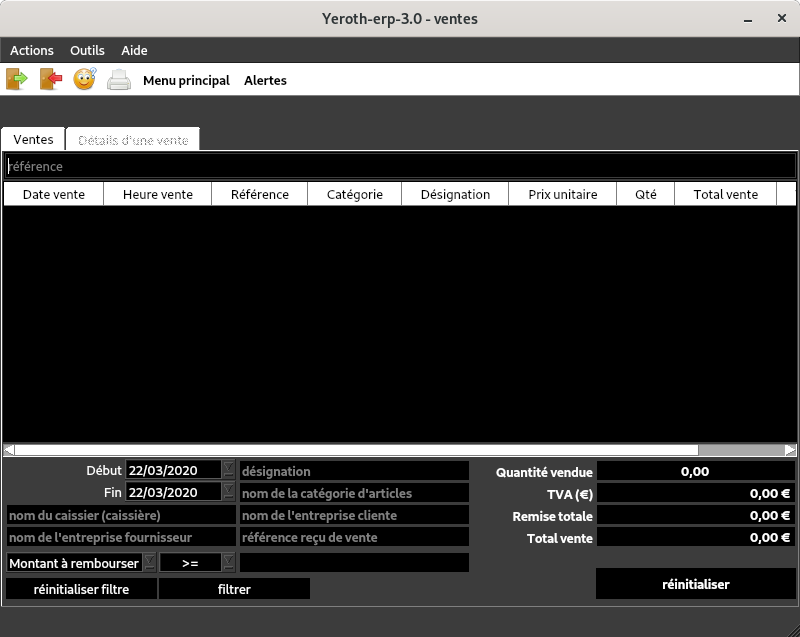
\includegraphics[scale=0.32]{../images/yeren-fenetre-caisse.png}
\caption{La fen\^etre des ventes}
\label{fig:fenetre-de-la-vente}
\end{figure}

\vspace{-1.9em}
\section{Les atouts de \yeren}
\vspace{-0.3em}
\begin{enumerate}[1)]
	\itemsep -0.3em
	\item une tr\`es grande stabilit\'e de l'application
	\item des utilisateurs avec des r\^oles bien sp\'ecifi\'es
	\item un syst\`eme d'alerte qui comporte des alertes
	      param\'etr\'ees en fonction des quantit\'es en stock
	      ou des p\'eriodes de temps
	\item la possibilit\'e de g\'en\'er\'er des re\c{c}us au
	      petit format pour des imprimantes thermiques, ou bien
	      de g\'en\'er\'er des documents au format ''A4''
	\item Linux--Debian comme syst\`eme d'exploitation, car
	      tr\`es stable, performant, et moins vuln\'erable
	      aux attaques des pirates informatiques en comparaison
	      aux autres syst\`emes d'exploitation
	\item une interface ''ventes'' qui permet au \manager
	      d'avoir une vue d'ensemble des 
	      ventes~(voir la Figure~\ref{fig:fenetre-de-la-vente}),
	      et aussi d'effectuer des ''retours sur ventes''
	\item une interface ''tableaux de bords'' qui
		  g\'en\`ere des rapports financiers,
		  pour l'aide \`a la d\'ecision manag\'eriale
		  du ''business''.
\end{enumerate}

\vspace{-1em}
\section{Le syst\`eme d'alerte}
\vspace{-0.5em}
Les utilisateurs aux r\^oles \administrateur ou
\manager sont ceux capable de cr\'eer des
alertes dans \yeren.
\yeren permet  de cr\'eer des alertes pour:
\begin{enumerate}[1)]
	\itemsep -0.5em
	\item une quantit\'e d'articles restante en stock
	\item une p\'eriode de temps.
\end{enumerate}

\vspace{-1em}

\subsection{Alertes sur une quantit\'e en stock}
\vspace{-0.1em}
Une alerte sur la quantit\'e en stock (X) d'un produit
est un message qui est g\'en\'er\'e lorsque la
quantit\'e en stock de ce produit atteint X.

Par exemple Xavier (\manager) cr\'ee une alerte sur le
produit ''mangue'' qui se d\'eclenche d\`es que sa quantit\'e
en stock atteint $100$; $1$ message est g\'en\'er\'e et
envoy\'e \`a l'utilisateur Jean (\magasinier).

\vspace{-1em}

\subsection{Alertes sur une p\'eriode de temps}
\vspace{-0.1em}
Une p\'eriode de temps est d\'efinie par $1$ date
de d\'ebut de p\'eriode, et $1$ date de fin
de p\'eriode.

Une alerte sur une p\'eriode de temps pour un
produit est un message qui est g\'en\'er\'e et 
qui reste existant dans \yeren durant toute la
dur\'ee de cette p\'eriode de temps.

Par exemple, un message d'alerte doit \^etre envoy\'e
a l'utilisateur Paul (\caissier) d\`es que
la date du $05$~Mai est atteinte afin que celui-ci
applique un rabais de $20\%$ sur chaque vente de
yaourt 'tr\`esbon' durant une p\'eriode de $2$ semaines.

\vspace{-1.1em}
\section{Le syst\`eme de gestion de base--de--donn\'ees}
\vspace{-0.3em}
\mariadb est utilis\'e comme syst\`eme de gestion
de base de donn\'ees. \mariadb est tr\`es stable,
tr\`es performant, et source--libre.

Des copies ex\'ecutables de \mariadb peuvent \^etre
accessible \`a tr\`es moindre co\^ut (ex.: $0$).

\vspace{-1.1em}
\section{Conclusion}
\vspace{-1em}
\begin{figure}[!htbp]
\centering
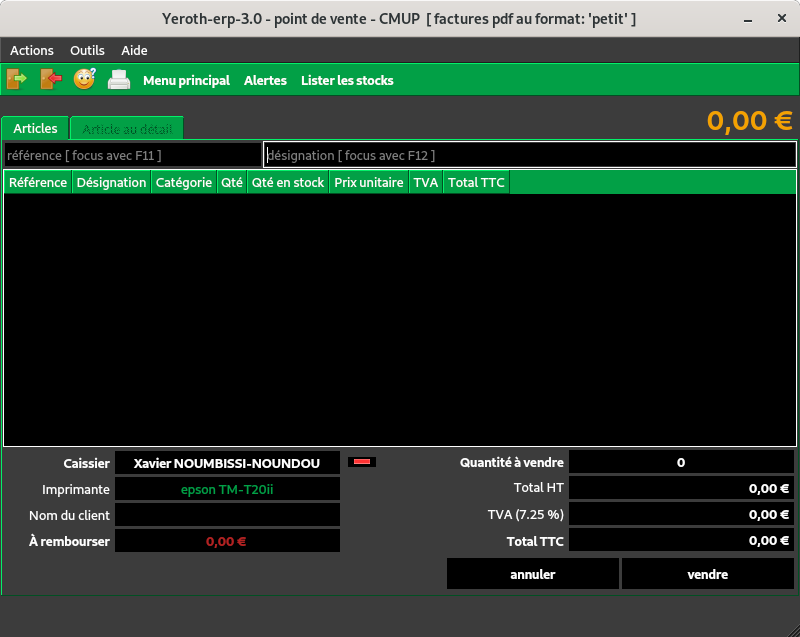
\includegraphics[scale=0.33]{../images/yeren-fenetre-caissier.png}
\caption{La fen\^etre de vente}
\label{fig:fenetre-de-vente}
\end{figure}

La Figure~\ref{fig:fenetre-de-vente} illustre la
fen\^etre pour faire les ventes d'articles.

\yeren est disponible dans les langues Anglais et Fran\c{c}ais. 

\end{document}
